\chapter{Descrição do Sistema ``Admins''}
\label{chap4}

Dado a escolha de um banco de dados em grafo como o Neo4j, o sistema ``Admins'' veio para resolver o problema de ser complicado e pouco seguro gerenciar os dados diretamente através de uma Cypher no banco, sendo facilmente possível realizar consultas muito pesadas, ou que tem consequências difíceis de reverter, de maneira acidental.

Foi então desenvolvido uma interface para usuários interagirem com o banco, podendo criar, editar, conectar e desconectar arbitrariamente nós no banco de dados. Esse sistema foi nomeado de 'admins', graças ao subdomínio utilizado para hospoedá-lo.

\section{Perfis e Listas}

Junto com o time de Design, identificamos uma maneira de entender e visualizar o grafo que está armazenado no banco, dando para cada nó uma página de perfil, que mostra e permite edição de suas propriedades e relações, além de uma página de lista/pesquisa para cada rótulo (relevante) no banco de dados. Endentendo este isomorfismo, conseguimos criar esta interface e permitir os usuários navegarem e editarem o grafo de maneira intuitiva.

\begin{figure}[H]
    \centering
    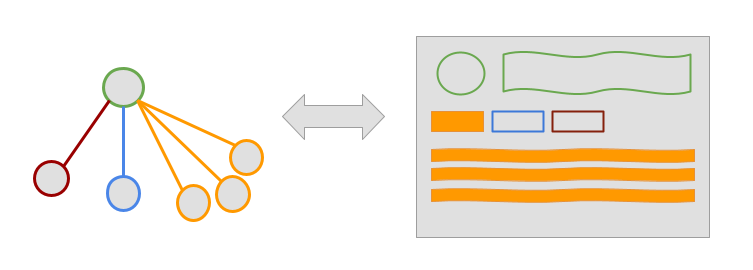
\includegraphics[width=1.0\linewidth]{Imagens/chap04/perfil-isomorfismo.png}
    \caption{Um \textcolor{green}{\textbf{nó X}} está relacionado à \textcolor{purple}{\textbf{um nó de rótulo Y}}, \textcolor{blue}{\textbf{um de rótulo W}}, e possui relação com \textcolor{orange}{\textbf{três nós de rótulos Z}} no grafo armazenado no banco de dados.}
    \label{fig:isomorphism}
\end{figure}


Temos então as propriedades do nó dono do perfil na parte superior da tela, e diferentes abas (uma para cada tipo de relação que o nó dono possui) na parte inferior, sendo que dentro de cada aba, uma lista de elementos com os nós vizinhos através daquele tipo de relação, com hiperlinks para páginas de perfis de seus vizinhos. Assim conseguimos andar pelo grafo através dos nós e relações, e em cada parada temos ações específicas como edição, criação ou conexão de nós.

Porém para o usuário começar esta navegação, ele precisa primeiro determinar o nó inicial. Essa é a função da chamada página de Lista, que como o nome sugere lista de maneira paginada e com funções de pesquisa os nós de algum rótulo específico, numa lista de elementos similar à uma aba dentro de um perfil. Permitindo agir sobre esses nós, ou entrar na página de perfil de um deles, começando a navegação pelos perfis.

A vantagem dessa modelagem é que conseguimos perceber que toda página de perfil (e de lista) segue a mesma regra, logo o código referente à sua implementação pode ser reutilizado. Ná prática a aplicação consiste em apenas uma página de perfil, e uma página de lista (além da página de login/autenticação), e mapas que definem as especificidades de cada caso, facilitando sua manutenção e minimizando o tamanho do seu código, consequentemente minimizando também bugs em produção.

\section{Arquitetura da Aplicação Cliente}

\subsection{Ações}

\section{Arquitetura do Servidor com endpoint GraphQL}

O frontend, entretando, não se comunica diretamente com o banco de dados, a interface se comunica com uma camada intermediária através de requisições em GraphQL, e esta camada intermediária gera a Cypher resultante, que então é executada no banco de dados. Nesta seção descreveremos como funciona e a arquitetura escolhida para esta camada intermediária, o servidor que disponibiliza a endpoint em Graphql.

 \begin{figure}[H]

\begin{tikzpicture}[font=\small,thick]
 
% Start block
\node[draw,
    rounded rectangle,
    minimum width=2.5cm,
    minimum height=1cm] (block1) { Interface do ``Admins'' };
 
% Voltage and Current Measurement
\node[draw,
    below=0.8cm of block1,
    minimum width=2.5cm,
    minimum height=1cm
] (block2) { Servidor (Node.js) com endpoint GraphQL };
 
% Power and voltage variation
\node[draw,
    below=0.8cm of block2,
    minimum width=2.5cm,
    minimum height=1cm
] (block3) { Banco de Dados (Neo4j) };

\draw (block1) |- (block2);
\draw (block2) |- (block3);

\end{tikzpicture}
\caption{Fluxograma de comunicação entre partes do sistema }
\label{chap3:fluxograma}
\end{figure}